\section{A simplified language}\label{sec:simple-language}

Section \ref{sec:RTEC-language} thoroughly discussed the features of the language of RTEC. In this section we will describe a simplified version of the RTEC language, and the Event Calculus, in general.

So far, in order to address an Event Recognition problem, the RTEC users need to be familiar with Prolog, and often have to take care to use several special, built-in predicates and functions -- e.g.: the interval manipulation constructs -- correctly. Another, simpler form of the Event Calculus, with its own compiler has been designed and developed. This simplified Event Calculus (SimplEC) aims at producing much simpler and readable Event Descriptions, even for demanding domains, and at the same time it maintains most of the expressiveness of RTEC.

The time model remains linear, with integer time points. What changes is the representation of the events and fluents, as well as the format of the rules within an Event Description.

First of all, SimplEC is not Prolog, in contrast with the classic RTEC event patterns. It is designed to resemble simple statements in English, with some pseudocode and mathematical elements. It does not contain obscure symbols like \texttt{:-}, or \texttt{\textbackslash +}. Instead, it contains simple words like \texttt{if}, \texttt{or}, \texttt{not}, as well as the comma operator that indicates conjunction. There are also a few special tokens, like \texttt{happens} that stem from the classic RTEC language.

\subsection{Representing events and fluents}

In this simplified version of the RTEC language, there are no special predicates like \texttt{holdsAt(F=V,T)}, \texttt{holdsFor(F=V, I)}, or \texttt{happensAt(E, T)} that indicate happening, holding, initiation and termination, as we have seen on the section about RTEC. All events and fluents are represented using a compound term of the form
%
\begin{align}
& \label{eq:compound_term}
\begin{mysplit}
\mathrm{functor}( \dots \mathit{arguments}\dots )[\val\mathit{value}]
\end{mysplit}
\end{align}
%
where square brackets denote the optional part of the term. This structure allows for the representation of both events and fluents. Specifically, when this term contains a value, then it is always a fluent. When the value is absent, it may either be a fluent with the default ``\texttt{true}'' value, or an event which, by definition, has no value. The distinction between the latter two categories is based on the context.

\subsubsection{Built-in tokens}

There are a handful of built-in keywords that precede the compound terms shown in \ref{eq:compound_term} and help identify how the term is being used. These keywords are:
\begin{itemize}
\item \texttt{initiate}: Indicates that the following term is a fluent and is being initiated. Similar to classic RTEC's $\initiatedAt$.
\item \texttt{terminate}: Indicates that the following term is a fluent and is being terminated. Similar to classic RTEC's $\terminatedAt$.
\item \texttt{start}: Denotes the point in time where the following fluent starts holding. Similar to classic RTEC's $\startE$.
\item \texttt{end}: Denotes the point in time where the following fluent ceases holding. Similar to classic RTEC's $\endE$.
\item \texttt{happens}: Indicates that the following term is an event and expresses its happening. Similar to classic RTEC's $\happensAt$.
\end{itemize}

\subsubsection{Defining simple fluents}

The SimplEC user can state initiation conditions for simple fluents as follows:
%
\begin{align}
& \label{eq:simple_fluent}
\begin{mysplit}
\mathbf{initiate}\ F_1\ \mathbf{if} \\
\qquad E[, \\
\qquad \mathrm{condition}]^*.
\end{mysplit}
\end{align}
%
Termination conditions are structured in the same way, the only difference being that instead of the keyword $\mathbf{initiate}$ we use the keyword $\mathbf{terminate}$.

$F_1$ is a fluent, following the syntax we have seen in \eqref{eq:compound_term}. $E$ can be either an ordinary event structured as in \eqref{eq:compound_term}, or one of the two special events ($\mathbf{start}\ F_2$, $\mathbf{end}\ F_2$), denoting the starting and ending points of the holding interval of another fluent $F_2$, respectively.

$[,\ \mathrm{condition}]^*$ denotes an optional set of conditions surrounding the happening of $E$, that are significant for the initiation or termination of $F_1$. Such a condition could be one of the following:
%
\begin{itemize}
\item $F_3$, meaning that fluent $F_3$ must hold at that specific timepoint.
\item $\mathbf{start}\ F_3$, meaning that $F_3$ must start holding.
\item $\mathbf{end}\ F_3$, meaning that $F_3$ must cease holding.
\item $\mathbf{not}\ F_3$, meaning that $F_3$ must not hold.
\item $\mathbf{happens}\ E_2$, indicating the happening of event $E_2$.
\item $\mathbf{not\ happens}\ E_2$, indicating the absense of event $E_2$.
\item atemporal constraint.
\end{itemize}

In the same fashion that we define the initiation and termination points of a simple fluent, we can also define the happening of events that are output entities. This can be achieved by replacing the $\mathbf{initiate}$ and $\mathbf{terminate}$ keywords with the $\mathbf{happens}$ keyword and putting an event instead of a fluent at the head of the statement. The body of the statement is structured exactly as in the initiation/termination case.

\subsubsection{Defining statically determined fluents}

A SimplEC statement defining a statically determined fluent consists of conjunctions, disjunctions and negations of other fluents, possibly nested within each other. The keyword $\mathbf{or}$ is used in disjunctions, the keyword $\mathbf{not}$ is used in negations, and conjunctions use the comma operator. There are no interval manipulation constructs, as the relevant information is contained in the occurrence of the respective operators and keywords.

The following example shows the definition of moving as a statically determined fluent. Two persons are considered to be moving together while they are both walking and they appear close to each other. This can be expressed in SimplEC as follows:
%
\begin{align}
& \label{eq:move-simplEC}
\begin{mysplit}
\mathit{moving(P_1, P_2)}\ \mathbf{if} \\
\qquad \mathit{walking(P_1),} \\
\qquad \mathit{walking(P_2),} \\
\qquad \mathit{close(P_1, P_2).}\\
\end{mysplit}
\end{align}

Another, more involved example is the definition of fighting. Fighting between two persons takes place when at least one of them is moving abruptly, none of them is totally inactive, and at the same time they are very close to each other. In SimplEC, we write:
%
\begin{align}
& \label{eq:fight-simplEC}
\begin{mysplit}
\mathit{fighting(P_1, P_2)}\ \mathbf{if}\\
\qquad \mathit{(abrupt(P_1)}\ \mathbf{or}\ \mathit{abrupt(P_2))},\\
\qquad \mathit{close(P_1, P_2)},\\
\qquad \mathbf{not}\ \mathit{(inactive(P_1)}\ \mathbf{or}\ \mathit{inactive(P_2))}.
\end{mysplit}
\end{align}

\subsection{Event Description}

An Event Description in SimplEC is a set of statements that follow the above-mentioned syntax. Let's consider a sample Event Description that only contains statements \eqref{eq:move-simplEC} and \eqref{eq:fight-simplEC}. It would look like this:

\begin{minipage}{\linewidth}
\lstinputlisting[
  style      = Prolog-cvlas,
  caption    = {Event description in SimplEC.},
  label	     = {lst:simplec-rules}
]{listings/simplec_rules.txt}
\end{minipage}

This set of rules translates into the following RTEC Event Description:

\begin{minipage}{\linewidth}
\lstinputlisting[
  style      = Prolog-cvlas,
  caption    = {Event description of Listing \ref{lst:simplec-rules} translated into RTEC.},
  label	     = {lst:rtec-rules}
]{listings/rtec_rules.txt}
\end{minipage}

\subsection{Declarations and Dependencies}

The compiler of SimplEC parses a set of statements in the simple language and, based on its grammar, translates the statements to rules in the RTEC format. Moreover, it constructs the declarations required for computing narrative assimilation queries. The declarations distinguish, for the benefit of RTEC, between simple and statically determined fluents, and between input and output entities (events and fluents). 
%The compiler parses each SimplEC statement and identifies each of the entities involved as an event, a simple fluent or a statically determined fluent, as well as deciding whether it is an input or an output entity. 
In SimplEC statement \eqref{eq:move-simplEC}, for instance, the compiler will detect three statically determined fluents, namely $\mathit{moving(\_,\_)}$, $\mathit{walking(\_)}$, and $\mathit{close(\_,\_)}$, of which $\mathit{moving(\_,\_)}$ is an output entity, as it appears in the head of the statement, and the other two are input entities, as they do not appear to be defined by other, simpler entities. This knowledge of the compiler is summarized in the following set of declarations:
%
\begin{align}
& \label{eq:move-decls}
\begin{mysplit}
\mathit{\textsf{\footnotesize sDFluent}(moving(\_, \_)).} \\
\mathit{\textsf{\footnotesize sDFluent}(walking(\_)).} \\
\mathit{\textsf{\footnotesize sDFluent}(close(\_, \_)).}\\
\mathit{\textsf{\footnotesize outputEntity}(moving(\_, \_)).} \\
\mathit{\textsf{\footnotesize inputEntity}(walking(\_)).} \\
\mathit{\textsf{\footnotesize inputEntity}(close(\_, \_)).}\\
\end{mysplit}
\end{align}

\begin{figure*}[t]
\centering
	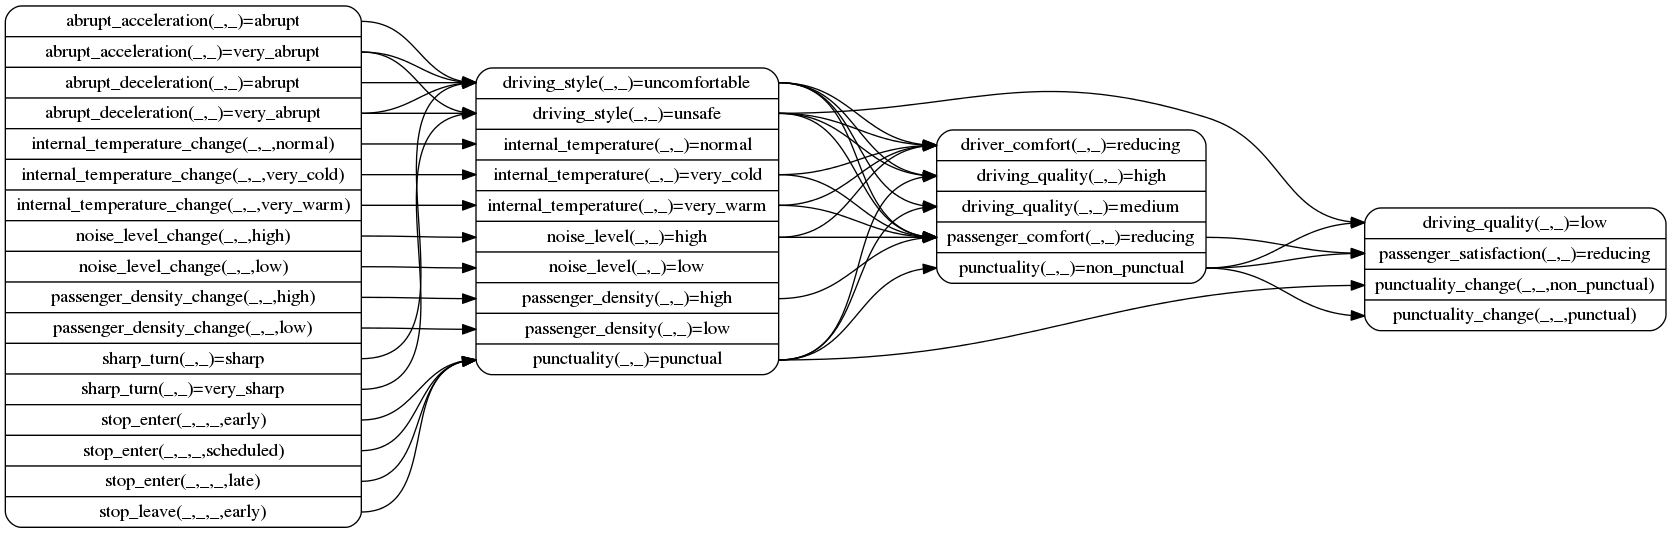
\includegraphics[width=\textwidth]{figures/ctm_graph.png}
	\caption{Dependency graph of the city transport management event description.}
	\label{fig:ctm_graph}
\end{figure*}

The declarations also express the `caching hierarchy', that is, the order in which fluents and events are processed. RTEC performs bottom-up processing whereby fluents and events of level 1 of a hierarchy are processed first, subsequently moving to levels 2, 3, etc. The computed intervals of each level are cached. This way, fluent and event intervals of some level $n$ may be simply fetched from memory when required in the processing of fluents and events of some higher level $m$.

To aid the user, the compiler may display the dependency graph of the event description. This is a directed graph where each vertex corresponds to a fluent or event, and for each pair of vertices $(i, j)$ there is an edge from $i$ to $j$ if $i$ appears in the body of a statement defining $j$. Figure \ref{fig:ctm_graph} shows the dependency graph of an event description for city transport management. In this figure, we can observe the way in which the events and fluents affect each other. In the leftmost part of the figure there are vertices with no incoming edges. These correspond to input events and fluents that form the narrative upon which all complex activities will be recognised. In this domain, the input entities include information about the acceleration and deceleration of  transport vehicles, changes in  internal temperature, noise level or passenger density, as well as the time of arrival at a stop.

On the right of the bottom layer, there are two other layers of events and fluents that have both incoming and outgoing edges. These are output entities that also contribute to the definition of other output entities. On these layers we combine information from the bottom layer and produce higher-level information. For instance, we can recognise complex activities such as driving style and quality, vehicle punctuality and the passengers' comfort level.
In the rightmost part of the figure, there is one last layer with no outgoing edges. These are the complex activities of the highest level---consider, for instance, passenger satisfaction.

\subsection{Running the compiler}

The compiler of the SimplEC language is written in Prolog and is based on Prolog's Definite Clause Grammars, which are often used for NLP purposes and building parsers, in general.

In order to use the compiler, the user must type:
{\small
\begin{verbatim}
   $ swipl -l simplEC.prolog
\end{verbatim}
}

And then, supposing that the user has written their set of SimplEC statements in a file named ``simplec\_rules.txt'', type:
{\small
\begin{verbatim}
   ?- simplEC('simplec_rules.txt', 'event_description.prolog',
                              'declarations.prolog', 'dependency_graph.txt').
\end{verbatim}
}
This will take the file with the event patterns in SimplEC and translate it to an Event description in the classic RTEC format, along with its respective declarations, as we have seen in detail, earlier in this manual. But before the Event Recognition process is started, the rules must be further compiled by the compiler of RTEC this time.

To save time and to unify the two compilation steps, there is an executable script named ``compile.sh'' that calls both compilers and produces the compiled event description and the declarations that are needed for RTEC to start performing Event Recognition. To call that script, the user should write in a command window:
{\small
\begin{verbatim}
   $ bash compile.sh simplec_rules.txt
\end{verbatim}
}
